\documentclass[10pt]{beamer}

\usetheme{Warsaw}
\beamertemplatenavigationsymbolsempty

\usepackage[utf8x]{inputenc}
\usepackage[francais]{babel}
\usepackage{hyperref}
\usepackage{amsmath}
\usepackage{graphicx}
\usepackage{tikz}
\usepackage{multicol}
\usetikzlibrary{automata,positioning}
\graphicspath{{./img/}}
\DeclareGraphicsExtensions{.png, .jpeg, .jpg}


\renewcommand*\thesection{\arabic{section}}

\hypersetup{
    colorlinks,
    citecolor=blue,
    filecolor=blue,
    linkcolor=blue,
    urlcolor=blue
}

\AtBeginSection[]{%
  \begin{frame}<beamer>
    \frametitle{Plan}
    \tableofcontents[sectionstyle=show/hide,subsectionstyle=hide/show/hide]
  \end{frame}
  \addtocounter{framenumber}{-1}
}

\setbeamertemplate{footline}[frame number]


\title{Statistical Machine Translation for Query Expansion in Answer
  Retrieval\cite{Riezler07}\\ 
\small
Stefan Riezler, Alexander Vasserman, Ioannis Tsochantaridis, Vibhu
Mittal and Yi Liu}

\author{Rémi Bois, Agathe Mollé}
\date{\today}

\begin{document}

\begin{frame}
  \maketitle
  \vfill
  \begin{figure}
    
\includegraphics[width=0.20\textwidth]{logo_univ_nantes}
  \end{figure}

\end{frame}

\begin{frame}
  \tableofcontents
\end{frame}

\section{Introduction}
\label{sec:intro}

\begin{frame}
  \frametitle{Introduction}
  \begin{block}{Problématique en Question Answering}
  Fossé lexical entre une question et sa réponse
  \begin{itemize}
    \item vocabulaire
    \item reformulation
    \item ambiguités du langage naturel
  \end{itemize}
  \end{block}
  
  \pause
  
  \begin{block}{Problématique en Recherche d'Information}
  Problématique similaire en RI sur la correspondance des termes entre la requ\^ete et les documents.
  
  $\implies$ Expansion de requ\^ete
  \end{block}
\end{frame}

\begin{frame}
  \frametitle{L'article}  
  \begin{block}{Statistical Machine Translation for Query Expansion in Answer Retrieval}
  \begin{itemize}
    \item Stefan Riezler, Alexander Vasserman, Ioannis Tsochantaridis, Vibhu Mittal and Yi Liu
    \item Google Inc.
    \item Proceedings ACL 2007
  \end{itemize}
  \end{block}
\end{frame}

\section{Question Answering}
\label{sec:QA}

\begin{frame}
  \frametitle{Répondre à des questions}
  % questions en langage naturel, réponses en langage naturel
  \begin{block}{Format}
    Les questions sont posées en langage naturel.

    Exemple : How to live with cat allergies ?

    Les réponses sont également données en langage naturel.
  \end{block}
\end{frame}

\begin{frame}
  \frametitle{Une tâche de Recherche d'Informations}
  % recherche dans un ensemble de FAQ

  \begin{block}{Comment répondre ?}
    On ramène la tâche de question/réponse à une recherche dans une
    base de FAQ. 

    Les documents retournés sont les réponses des
    questions d'une FAQ.
  \end{block}
\end{frame}

\section{Ajout de la paraphrase et de la traduction de questions}
\label{sec:paratrans}

\begin{frame}
  \frametitle{Reformulation de la question}
  % présenter l'intuition et un exemple
  \begin{block}{Améliorer la précision}
  La requête seule peut ne pas suffire à trouver la réponse adéquate.
  
  Il est donc judicieux de l'étendre à l'aide de reformulations du même problème.
  
  $\implies$ Utilité des paraphrases
  \end{block}
  \pause

  \begin{block}{Technique utilisée en QA}
    La reformulation, par variations syntaxiques (Hermjakob
    \cite{Hermjakob02} ou Lin \cite{Lin01}), ou par remplacement de
    termes via des ontologies (Burke \cite{Burke97}), ont déjà été
    explorées pour la tâche de Question Answering.
  \end{block}
\end{frame}

\begin{frame}
  \frametitle{Comment paraphraser ?}
  % double traduction
  \begin{block}{Approche utilisée}
  \begin{itemize}
    \item Utilisation d'une langue pivot pour identifier des paraphrases/synonymes
    \item Double traduction d'expressions, groupes de mots
    \item Passage par autant de langues pivots que possible, puis sélection des meilleurs résultats
    \item Expansion de requête en ajoutant les termes introduits par les n-meilleures paraphrases de la requête
  \end{itemize}
  \end{block}
\end{frame}

\begin{frame}
  \frametitle{Sélection des paraphrases}
  %formule
  \begin{block}{Sélection des n-meilleures paraphrases}
  La probabilité de paraphrase d'une phrase complète est obtenue en faisant un produit, pour tous les constituants (groupes de mots) de la phrase des :
  \begin{itemize}
    \item fréquences relatives des constituants dans les tables bilingues
    \item fréquences relatives des mots dans les tables bilingues
    \item nombre de constituants
    \item nombre de mots
    \item score de \textit{reordering}
    \item score associé à un modèle de langue 6-gramme
  \end{itemize}
  \end{block}
\end{frame}

\begin{frame}
  \frametitle{La traduction automatique pour améliorer les résultats
    ?}
  % traduction question -> réponse + exemple
  \begin{block}{Autre utilisation de la traduction automatique}
  On considère les questions et les réponses comme deux langages distincts $\implies$ corpus parallèle
  
  La traduction d'une question en réponse va permettre d'apprendre les associations entre certains mots de la questions et leurs synonymes dans la réponse.
  \end{block}
\end{frame}

\begin{frame}
  \frametitle{Exemple}
  \begin{figure}[h]
    \centering
    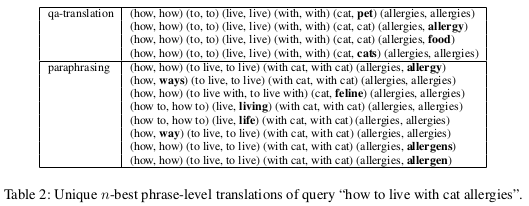
\includegraphics[width=\textwidth]{table2}
    \label{fig:res}
  \end{figure}
\end{frame}

\section{Corpus et données d'entraînement}
\label{sec:corpus}

\begin{frame}
  \frametitle{L'entraînement du module de paraphrase}
  % russe truc
  \begin{block}{Données d'entra\^inement}
    Traductions manuelles Chinois$\rightarrow$Anglais (NIST 2006)
    
    $\implies$ Une table de paraphrases comprenant 33 millions de paires de paraphrases en anglais, extraite à partir d'un milliard de paires de constituants.
  \end{block}
\end{frame}

\begin{frame}
  \frametitle{Le corpus composé de FAQ}
  % présentation du corpus, stats etc...
  \begin{block}{Corpus}
  \begin{itemize}
    \item 4 milliards de pages web crawlées
    \item 2.6 millions de pages extraites avec les requ\^etes \og \verb?inurl:faq? \fg{} et \og \verb?inurl:faqs? \fg{} 
  	\item étiquetage manuel de 1000 pages pour entraîner un classifieur obtenant 90\% de score F1 $\implies$ 795 486 pages considérées comme FAQ
  	\item Extraction des questions/réponses brutale pour avoir la meilleure précision possible (ponctuation, tags HTML, marqueurs (ex: Q:, (1)) et ancres lexicales) $\implies$ 10 millions de paires question/réponse
  	\item Evaluation manuelle sur 100 documents atteignant une précision de 98\%.
  \end{itemize}
  \end{block}
\end{frame}


\section{Résultats}
\label{sec:results}


\begin{frame}
  \frametitle{Les données de test}
  \begin{block}{Données}
    20 réponses évaluées pour chacune des 60 questions posées.
  \end{block}

  \pause

  \begin{block}{Evaluation}
    2 juges, avec discussion lors d'un désaccord.
    
    Jugement en 3 critères :
    \begin{description}
    \item[adéquat] La réponse est contenue dans le document retourné
    \item[matériel] Pas de réponse exacte mais des informations importantes
    \item[insatisfaisant] Le besoin d'information de l'utilisateur
      n'est pas satisfait.
    \end{description}
  \end{block}
\end{frame}

\begin{frame}
  \frametitle{Baseline}

  \begin{block}{Mesure tfidf}
    La requête est lancée et les résultats retournés sont calculés
    avec une mesure tfidf classique.
  \end{block}
  \pause

  \begin{block}{Local expansion}
    Correspond à une extension de requête locale classique :

    \begin{itemize}
    \item La requête est lancée une première fois
    \item Les termes les plus importants (tfidf) des premiers
      documents retournés sont ajoutés à la requête
    \item La requête est relancée avec les termes originaux et les
      nouveaux termes
    \end{itemize}
  \end{block}
  % description de la baseline
  % description du S_2@n
\end{frame}

\begin{frame}
  \frametitle{Les détails du tfidf utilisés}

  \begin{block}{Vecteur de poids}
    \begin{figure}[h]
      \centering
      $<0.0, 1.0, 0.0, 0.0, 0.5, 0.5, 0.2, 0.3>$
    \end{figure}
    
    
    Les poids du vecteurs correspondent à :

    \begin{enumerate}
    \item Le texte de tout le document
    \item Le texte de la question
    \item Le texte de la réponse
    \item Le texte du titre
    \item Chacun des textes ci-dessus, sans les stopwords
    \end{enumerate}

    Le but du second poids est de prendre en compte les termes
    interrogatifs (when, where, which, ...)

  \end{block}
  \pause
  \begin{block}{La mesure utilisée}
    Comparaison des vecteurs via la mesure Cosine
  \end{block}

\end{frame}

\begin{frame}
  \frametitle{Résultats}
  % le tableau
  \begin{figure}[h]
    \centering
    \begin{tabular}[h]{|c|c|c|c|c|}
    \hline
    & $S_2@10$ & $S_2@20$ & $S_{1,2}@10$ & $S_{1,2}@20$\\
    \hline
    baseline tfidf & 27 & 35 & 58 & 65\\
    local expansion & 30 (+11.1) & 40 (+14.2) & 57 (-1) & 63 (-3)\\
    SMT-based expansion & 38 (+40.7) & 43 (+22.8) & 58 & 65\\
    \hline
  \end{tabular}

    \caption{Résultats}
    \label{fig:res}
  \end{figure}

\end{frame}

\begin{frame}
  \frametitle{Explication des résultats}

  \begin{figure}[h]
    \centering
    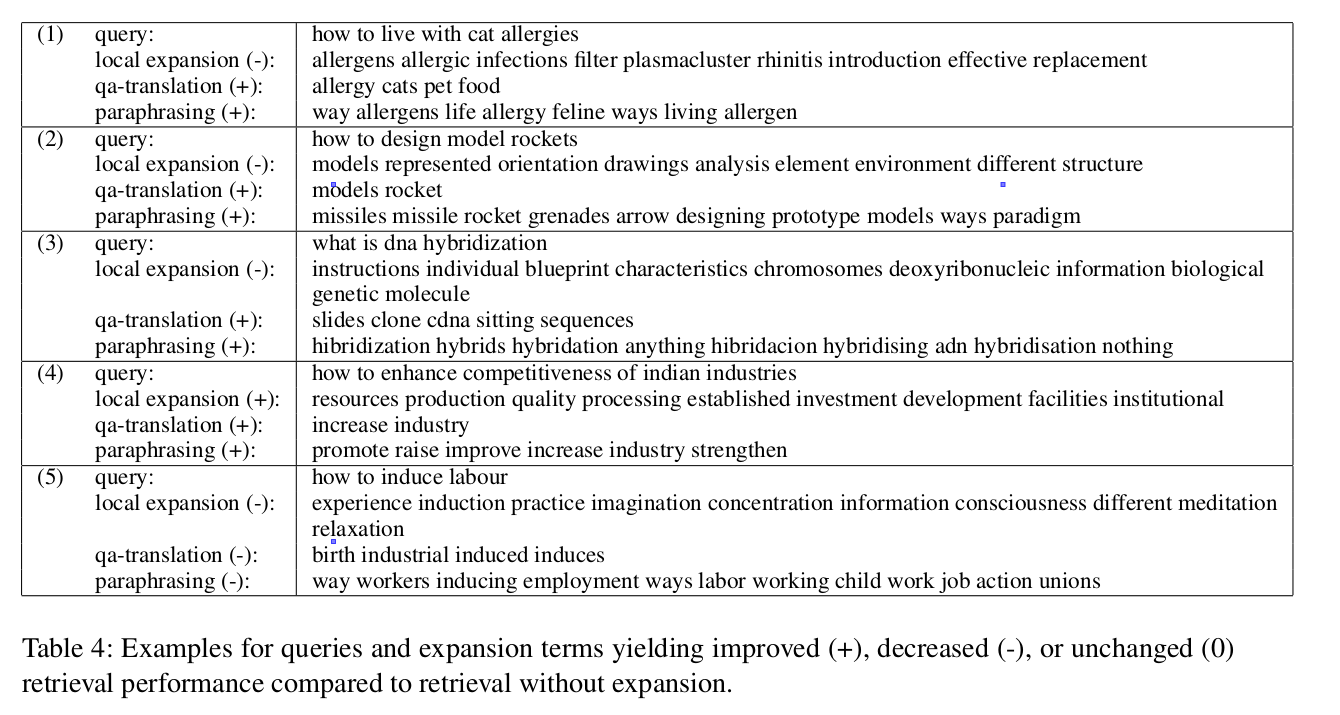
\includegraphics[width=\textwidth]{table4}
    \label{fig:res}
  \end{figure}
  % tableau 4 de l'article
\end{frame}

\section{Conclusion}
\label{sec:conclusion}


\begin{frame}
  \frametitle{Une méthode efficace}
  % approche nouvelle (?)
  \begin{itemize}
    \item Une approche nouvelle
    \item Les 2 techniques à base de SMT améliorent les baselines (tfidf et expansion locale de requ\^ete)
    \item Application limitée (FAQ) mais portable à de la Recherche d'Information plus générale
  \end{itemize}
\end{frame}

\begin{frame}
  \frametitle{Quelques limites}

  \begin{block}{Stemming}
  Il semble que beaucoup de termes retrouvés par la méthode de
  paraphrase et de traduction correspondent en fait à des variations
  du même terme (eg. allergens, allergy, allergies, ...). Un stemming
  aurait permis de lever ces ambiguïtés sans avoir à recourir à ce système.
  \end{block}
  \begin{block}{Taille de l'évaluation}
    L'évaluation donne une idée de la précision, mais pas du rappel.
    
    On ne connaît pas le nombre de discussions nécessaires entre les
    juges pour trouver un accord.
  \end{block}
  % stemming ? taille du corpus de test ?
\end{frame}


\begin{frame}[allowframebreaks]
  \frametitle{Références}
  \bibliographystyle{amsalpha}
  \bibliography{pres.bib}
\end{frame}

\end{document}